\documentclass{article}

% \usepackage{draftwatermark}
% \SetWatermarkText{Draft}
% \SetWatermarkScale{5}
% \SetWatermarkLightness {0.9} 
% \SetWatermarkColor[rgb]{0.7,0,0}


\usepackage{geometry}                		% See geometry.pdf to learn the layout options. There are lots.
\geometry{letterpaper}                   		% ... or a4paper or a5paper or ... 
%\geometry{landscape}                		% Activate for for rotated page geometryhttps://www.washingtonpost.com/world/europe/amid-impeachment-probe-gordon-sondland-is-overseeing-a-renovation-of-his-residence-that-has-cost-1-million-in-taxpayer-money/2019/10/16/d0eece92-ef86-11e9-bb7e-d2026ee0c199_story.html?tid=sm_tw
%\usepackage[parfill]{parskip}    		% Activate to begin paragraphs with an empty line rather than an indent
\usepackage{graphicx}				% Use pdf, png, jpg, or eps� with pdflatex; use eps in DVI mode
								% TeX will automatically convert eps --> pdf in pdflat						\label{thm:integral_domain}

								% TeX will automatically convert eps --> pdf in pdflatex		
\usepackage{amssymb}
\usepackage{amsmath}
\usepackage{amsthm}
\usepackage{mathrsfs}
\usepackage[hyphens,spaces,obeyspaces]{url}
\usepackage{url}
\usepackage{hyperref}
\usepackage{subcaption}
\usepackage{authblk}
\usepackage{mathtools}
\usepackage{graphicx}
\usepackage[export]{adjustbox}
\usepackage{fixltx2e}
\usepackage{hyperref}
\usepackage{alltt}
\usepackage{color}
\usepackage[utf8]{inputenc}
\usepackage[english]{babel}
\usepackage{float}
\usepackage{bigints}
\usepackage{braket}
\usepackage{siunitx}
\usepackage{mathtools}


\usepackage{tikz}
\usepackage{verbatim}
\usetikzlibrary{plotmarks}
\usepackage{pgfplots}
\usepackage{amsmath}
\usepackage{relsize}
 \usepackage[hyphenbreaks]{breakurl}
 
 \newtheorem{thm}{Theorem}[section]
% \newtheorem{defn}[thm]{Definition}
\theoremstyle{definition}
\newtheorem{definition}{Definition}[section]
\newtheorem{proposition}{Proposition}[section]
\newtheorem{lemma}{Lemma}[section]
\newtheorem{example}{Example}[section]

\newcommand{\argmax}{\operatornamewithlimits{argmax}}
\newcommand{\argmin}{\operatornamewithlimits{argmin}}




\title{A Few Notes On The Dirac Delta Function And \\ The Laplace Transform}
\author{David Meyer \\ dmm@1-4-5.net}

\date{Last update: \today}							% Activate to display a given date or no date

\begin{document}
\maketitle

\section{Introduction}
These notes began life as some thoughts on the Dirac Delta Function and evolved into notes on several related topics including  Laplace Transforms. The 
Dirac Delta function has all kinds of crazy and interesting properties. More TBD.

\section{The Dirac Delta Function}
The Dirac Delta Function is defined as shown in Figure \ref{fig:delta}. In the limit ($\mathlarger{\epsilon} \to 0$) the
 Dirac Delta function is written $\delta_a(t)$ or sometimes $\delta(t - a)$. As we will see in a moment, the $\delta_{a,\epsilon}(t)$ form of the delta function
 is useful when we want to use the Mean Value Theorem for Integrals \cite{wiki:meam_value_theorem_for_integrals} to evaluate integrals involving the delta function.
 
\bigskip

\begin{figure}[H]
  \centering
  \begin{tikzpicture}[scale=1.7]
     \draw [<->] (0,3) -- (0,0) -- (4,0);                                                                      % draw axes
     \draw (3,2) node[rectangle] {                                                                           % draw function to the right
         $\delta_{a,\epsilon}(t) =  
           \begin{cases} 
             \frac{1}{\mathlarger {\epsilon}} & a \leq t \leq a + \epsilon \\
             0                                               & \text{otherwise}
           \end{cases}$
       }; 
     \draw [dashed] (1,0) node[below] {$a$}                 -- (1,1); 
     \draw [dashed] (2,0) node[below] {$a + \epsilon$} -- (2,1);
     \coordinate (y) at (0,1); \fill [black] (y) circle (1pt);                                           % draw a dot on the y axis (I'd like to make it smaller but I don't see how)
     \draw (0,1) node[left] {$\frac{1}{\mathlarger{\epsilon}}$};
     \draw [thick,red] (0,0) -- (1,0);
     \draw [thick,red] (2,0) -- (4,0);
     \draw [thick,red] (1,1) -- (2,1);
     \draw [dashed]   (0,1) -- (1,1);
     \draw (4,0) node [label=right:{$t$}] {};
     \draw (0,3) node [label=above:{$\delta_{a,\epsilon}(t)$}] {};
  \end{tikzpicture}
  \caption{The Dirac Delta Function $\delta_{a,\epsilon}(t)$}
  \label{fig:delta}
\end{figure}

\bigskip
\noindent
So $\delta_{a,\epsilon}(t)$ is defined to be

\begin{equation*}
\delta_{a,\epsilon}(t) =  
 \begin{cases} 
      \frac{1}{\mathlarger {\epsilon}} & a \leq t \leq a + \epsilon \\
      0                                               & \text{otherwise}
   \end{cases}
\label{eqn:delta}
\end{equation*}

\noindent
\bigskip
and has the constraint that


\begin{equation*}
  \int_{0}^{\infty} \delta_{a,\epsilon}(t) =  1
\end{equation*}

\bigskip
\bigskip
\noindent
\bigskip
That is, $\delta_{a,\epsilon}(t)$ is in some sense a probability density.

\bigskip
\noindent
In the limit the Dirac Delta Function looks like

\begin{equation*}
\lim_{\epsilon \to 0} \delta_{a,\epsilon}(t) =
\delta_{a}(t) =  
 \begin{cases} 
     \infty & t = a\\
      0     & t \neq a
   \end{cases}
\end{equation*}

\bigskip
\noindent
or sometimes

\begin{equation*}
\delta (t - a) =  
  \begin{cases} 
        \infty & t = a \\
        0       & t \neq a
  \end{cases}
\end{equation*}

\bigskip
\noindent
$\delta_a(t)$ also has the constraint that 


\begin{equation*}
  \int_{0}^{\infty} \delta_{a}(t) =  1
\end{equation*}

\bigskip
\noindent
and so is also a probability density. $\delta_a(t)$  is shown in Figure \ref{fig:delta_limit}.

\bigskip
\begin{figure}[H]
  \centering
  \begin{tikzpicture}[scale=2.0]
     \draw [<->] (0,2) -- (0,0) -- (4,0);                                                                      % draw axes
     \draw (3,1) node[rectangle] {                                                                           % draw function to the right
         $\delta_{a}(t) =  
           \begin{cases} 
              \infty & t = a  \\
               0      & \text{otherwise}
           \end{cases}$
       }; 
     \draw (1,0) node[below] {$a$};
     \draw [dashed,red] (1,0) -- (1,2);
     \draw (4,0) node [label=right:{$t$}] {};
     \draw (0,2) node [label=above:{$\delta_{a}(t)$}] {};
     \draw [thick,red] (0,0) -- (1,0);
     \draw [thick,red] (1,0) -- (4,0);
  \end{tikzpicture}
  \caption{The Dirac Delta Function $\delta_{a}(t)$}
  \label{fig:delta_limit}
\end{figure}


\subsection{Integrals involving $\delta_{a,\epsilon}(t)$}
$\delta_{a,\epsilon}(t)$ has all kinds of interesting properties. One of them involves the integral of the product $\delta_{a,\epsilon}(t)$ with some function $g(t)$.  
Here we would like to evaluate integrals of the form

\bigskip
\begin{equation}
  \int_{0}^{\infty} \delta_{a,\epsilon}(t) g(t) dt
  \label{eqn:delta_integral}
\end{equation}

\bigskip
\noindent
where $g(t)$ is continuous on the interval $[a, a+\epsilon]$. 
 
\bigskip
\noindent
The Mean Value Theorem for Integrals  \cite{wiki:meam_value_theorem_for_integrals}  tells us that

\begin{equation}
  \int_{a}^{b} g(t) dt = (b -a) g(c)
  \label{eqn:mvti}
\end{equation}

\bigskip
\noindent
where the point $c$ lies in the interval $[a, a+\epsilon]$. Now, since we know that $\delta_{a,\epsilon}(t)$ is zero everywhere except on the interval
$[a, a+\epsilon]$ we can rewrite the improper integral in Equation \ref{eqn:delta_integral} as the proper integral

\begin{equation*}
  \int_{a}^{a + \epsilon} \delta_{a,\epsilon}(t) g(t) dt
\end{equation*}

\bigskip
\noindent
Here we can notice that $ \delta_{a,\epsilon}(t) = \frac{1}{\mathlarger{\epsilon}}$ on the interval $[a, a+\epsilon]$ so we can rewrite our integral as 

\bigskip
\begin{equation*}
  \int_{a}^{a + \epsilon} \frac{1}{\mathlarger{\epsilon}} g(t) dt =  \frac{1}{\mathlarger{\epsilon}} \int_{a}^{a + \epsilon} g(t) dt
\end{equation*}

\bigskip
\noindent
Now we can use Equation \ref{eqn:mvti}, the Mean Value Theorem for Integrals\footnote{This is where the $\delta_{a,\epsilon}(t)$ form of the delta function comes in handy.},
by setting $b = a + \epsilon$ and $a = a$ so that $b - a = \epsilon$. Then 

\bigskip
\begin{equation*}
 \frac{1}{\mathlarger{\epsilon}} \int_{a}^{a + \epsilon} g(t) dt =  \frac{1}{\mathlarger{\epsilon}} \underbrace{ \Big [(a + \epsilon) - a \Big]}_{b -a} g(c) = \frac{1}{\mathlarger{\epsilon}} \epsilon g(c) = g(c)
\end{equation*}

\bigskip
\noindent
where $c \in [a, a + \epsilon]$. 

% \newpage
\bigskip
\noindent
Finally, if we look at what happens to $c$ as $\epsilon \to 0$ we see that $\lim\limits_{\epsilon \to 0} c = a$ (sorry about the notation abuse)
so that 

\begin{equation}
  \int_{0}^{\infty} \delta_{a}(t) g(t) dt = g(a)
  \label{eqn:g(a)}
\end{equation}

\bigskip
\noindent
Essentially $\delta_{a}(t)$ pulls out the value of $g$ at $a$, that is, $g(a)$.

\bigskip
\noindent
Another way to get this result \cite{youtube:suskind2008.4} is to notice that the integrand of 

\bigskip
\begin{equation*}
  \int_{0}^{\infty} \delta (t-a) g(t) dt
\end{equation*}

\bigskip
\noindent
is zero everywhere except where $t = a$, so we can rewrite our integral as
 $\int_{0}^{\infty} \delta (t-a) g(a) dt = g(a) \int_{0}^{\infty} \delta (t-a) dt$ (since $g(a)$ doesn't depend on $t$). 
 Then since by definition $ \int_{0}^{\infty} \delta (t-a) dt = 1$ we get

\bigskip
\begin{equation*}
  \int_{0}^{\infty} \delta (t-a) g(t) dt = g(a)
\end{equation*}

\bigskip
\section{The Laplace Transform}
We start by defining the integral transform of some function $f(t)$.

\bigskip
\begin{definition} 
{\bf Integral Transform:} If a function $f(t)$ is defined on $[0,\infty)$ then we can define an integral transform to be the improper integral
\end{definition}

\begin{equation*}
F(s) = \int_0^\infty K(s,t) f(t) dt
\end{equation*}

\bigskip
\noindent
If the improper integral converges then we say that $F(s)$ is the \emph{integral transform} of $f(t)$. The function $K(s,t)$ is called the \emph{kernel}
of the transform. When $K(s,t) = e^{-st}$ the transform is called the {\bf Laplace Transform}.

\bigskip
\begin{definition} 
{\bf Laplace Transform:} The Laplace Transform of a function $f(t)$ is defined to be
\label{def:laplace_transform}
\end{definition}


\begin{equation}
\mathcal{L}\{f(t)\} = F(s) = \int_0^\infty e^{-st} f(t) dt
\label{eqn:laplace_transform}
\end{equation}

\bigskip
\noindent
The Laplace Transform will turn out to be useful when solving ordinary differential equations (ODEs). Interestingly, the Laplace Transform of the 
Dirac Delta Function turns out to be

\bigskip
\begin{equation*}
\begin{array}{lllll}
\mathcal{L}\{\delta_a(t)\} 
&=& \int_0^\infty  e^{-st} \delta_a(t) dt    &\qquad \qquad \mathrel{\#} \text{Equation \ref{eqn:laplace_transform} with $f(t) = \delta_a(t)$}                    \\  
[4pt]                                                        % get a bit of space
&=& \int_0^\infty g(t) \delta_a(t) dt         &\qquad \qquad \mathrel{\#} \text{set $g(t) = e^{-st}$}                                                                                      \\
[4pt]                                                        % get a bit of space
&=& g(a)                                                &\qquad \qquad \mathrel{\#} \text{by Equation \ref{eqn:g(a)}}                                                                           \\
[4pt]                                                        % get a bit of space
&=& e^{-sa}                                            &\qquad \qquad \mathrel{\#} g(a) = e^{-sa}
\end{array}
\end{equation*}

\subsection{The Linearity Property of the Laplace Transform}
\label{subsec:linearity}


\bigskip
\begin{definition} 
{\bf Linearity Property:} $\mathcal{L}\{af (t) + bg(t)\} = a\mathcal{L}\{f(t)\} + b\mathcal{L}\{g(t)\}$
\label{def:linearity_properity}
\end{definition}

\bigskip
\noindent
Interestingly, $\mathcal{L}$ is what is called a linear operator in vector space parlance \cite{wiki:linear_map}. 

\bigskip
\noindent
All good, but why does $\mathcal{L}$ have this property? Here's one way to think about it:

\smallskip
\begin{equation*}
\begin{array}{lllll}
\mathcal{L}\{af(t) + bg(t)\} 
&=& \int_0^\infty e^{-st} \big [af (t) + bg(t) \big] dt                                & \mathrel{\#} \text{definition of the Laplace Transform (Definition \ref{def:laplace_transform})}                               \\  
[10pt]                                                                                                   % get a bit of space
&=& \int_0^\infty e^{-st} af (t)  dt + \int_0^\infty e^{-st}  bg(t)  dt          & \mathrel{\#} \text{by the linearity of improper integrals \cite{lewis2014}}                                                                 \\
[10pt]                                                                                                   % get a bit of space
&=& a \int_0^\infty e^{-st}  f(t) dt + b \int_0^\infty e^{-st}  g(t) dt          & \mathrel{\#} \text{neither $a$ or $b$ depends on $t$}                                                                                            \\
[10pt]                                                                                                   % get a bit of space
&=& a \mathcal{L}\{f(t)\}  + b \mathcal{L}\{g(t)\}                                   & \mathrel{\#} \text{definition of the Laplace Transform (Definition \ref{def:laplace_transform})}
\end{array}
\end{equation*}



\smallskip
\subsection{So does every function have a Laplace Transform?}
The answer is no (consider a function like $f(t) = t^{-1}$). OK, then what are the properties that $f(t)$ must have in order to have a Laplace Transform? First, $f$ must
be of "exponential order". 


\bigskip
\begin{definition} 
{\bf Exponential Order:} A function $f$ is said to be of exponential order $c$ if there exist constants $c, M, \text{ and } T > 0$ such that $|f(t)| \leq Me^{ct}$ for all $t > T$.
\label{def:exponential_order}
\end{definition}

\bigskip
\noindent
Said another way, in order for $f(t)$ to be of exponential order $c$ we require that  

\bigskip
\begin{equation*}
\lim\limits_{t \to \infty} \frac{f(t)}{e^{ct}} = 0
\end{equation*}

\medskip
\bigskip
\noindent
Basically this is saying that in order for $f(t)$ to have a Laplace Transform then in a race between $|f(t)|$ and $e^{ct}$ as $t \to \infty$ $e^{ct}$ must
approach its limit first. This situation is depicted in Figure \ref{fig:exponential_order}.

\bigskip
\bigskip
\begin{figure}[H]
\center{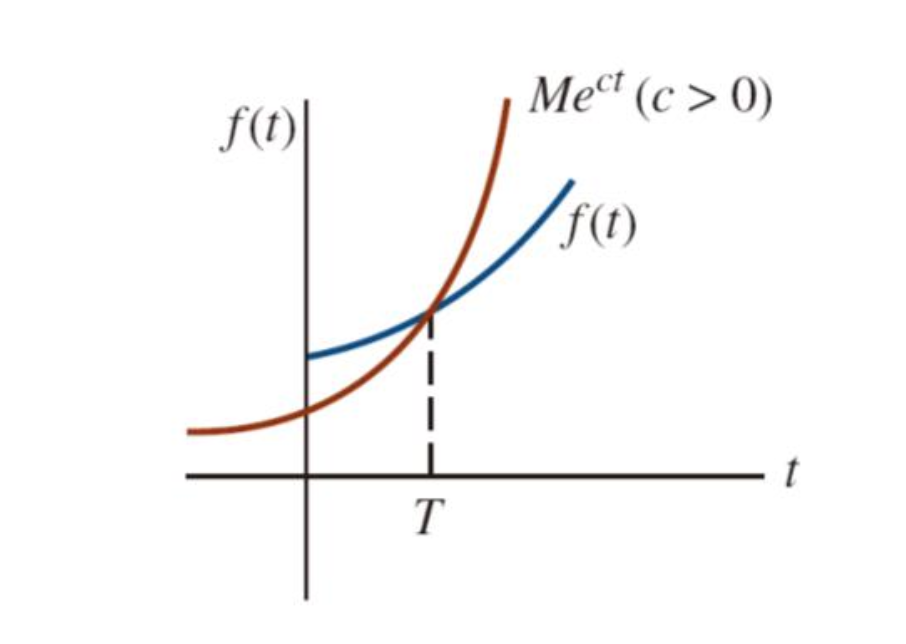
\includegraphics[scale=0.39,frame] {images/exponential_order.png}}
\caption{$f$ is of exponential order with constants $c, M$ and $T$}
\label{fig:exponential_order}
\end{figure}

\bigskip
\bigskip
\noindent
Now we can answer the question of when $f$ has a Laplace Transfrom:

\bigskip
\begin{thm} 
{\bf Existence Theorem for Laplace Transforms:} \normalfont If $f$ is s piecewise continuous on the interval $[0,\infty)$ and is of exponential order $c$ then 
$F (s) = \mathcal{L}\{f (t)\} \text{ is defined for all $s > c$}.$
\end{thm}

\bigskip
\noindent
Ok, but why? Consider

\begin{equation*}
\begin{array}{lllll}
\mathcal{L}\{f(t)\}
&=& F(s)                                                                            &\quad  \mathrel{\#} \text{definition of the Laplace Transform (Definition \ref{def:laplace_transform})}                                                \\  
[12pt]                                                                                 % get a bit of space
&=&   \mathlarger{\int}_0^\infty \! e^{-st} f(t) dt                  &\quad  \mathrel{\#} \text{definition of the Laplace Transform (Definition \ref{def:laplace_transform})}                                                \\  
[12pt]                                                                                 % get a bit of space
&\leq& \mathlarger{\int}_0^\infty \! e^{-st}  Me^{ct}dt         &\quad  \mathrel{\#} \text{$f$ is of exponential order $c$ (Definition \ref{def:exponential_order})}                                                      \\  
[12pt]                                                                                 % get a bit of space               
&=& M \mathlarger{\int}_0^\infty \! e^{-st} e^{ct} dt           &\quad  \mathrel{\#} \text{$M$ doesn't depend on $t$}                                                                                                                          \\   
[12pt]                                                                                % get a bit of space
&=& M \mathlarger{\int}_0^\infty \! e^{-st + ct}  dt             &\quad  \mathrel{\#} \text{$x^n \cdot x^m = x^{n+m}$}                                                                                                                           \\      
[12pt]                                                                                 % get a bit of space
&=& M \mathlarger{\int}_0^\infty\! e^{(c-s)t}  dt                 &\quad  \mathrel{\#}  e^{-st + ct} = e^{ct -st} = e^{(c-s)t}                                                                                                                        \\      
[12pt]                                                                                 % get a bit of space
&=&  M \mathlarger{\int}_0^\infty \! e^u dt                         &\quad  \mathrel{\#} \text{use a $u$ substitution with $u = (c-s)t$}                                                                                                       \\     
[12pt]                                                                                 % get a bit of space
&=&  M \mathlarger{\int}_0^\infty \! e^u \frac{du}{c-s}       &\quad  \mathrel{\#} u = (c-s)t  \: \Rightarrow \: du = (c-s) dt \: \Rightarrow \: dt = \dfrac{du}{c-s}                                                         \\     
[12pt]                                                                                % get a bit of space
&=& \Big [ \frac{M}{c-s} \Big ] \mathlarger{\int}_0^\infty \! e^u du                                    &\quad  \mathrel{\#} \text{neither $c$ or $s$ depends on $t$}                                                                \\     
[12pt]                                                                                % get a bit of space
&=& \Big [ \frac{M}{c-s} \Big ] e^u \Big |_0^\infty              &\quad  \mathrel{\#} \int_0^\infty e^u du = e^u +C \text{ and the Fundamental Theorem of Calculus}                                                  \\     
[12pt]                                                                                % get a bit of space
&=& \Big [ \frac{M}{c-s} \Big ]  e^{(c-s)t} \Big |_0^\infty     &\quad  \mathrel{\#} u = (c-s)t                                                                                                                                                                \\
[12pt]                                                                                % get a bit of space     
&=& \lim\limits_{d \to \infty}\Big [\frac{M}{c-s} e^{(c-s)d} \Big ] - \frac{M}{c - s}e^{(c-s)0}  &\quad \mathrel{\#} \text{evaluate at the limits}                                                                                     \\
[12pt]                                                                                % get a bit of space
&=& \lim\limits_{d \to \infty}\Big [\frac{M}{c-s} e^{(c-s)d} \Big ] - \frac{M}{c - s}                 &\quad  \mathrel{\#} e^{(c-s)0} = e^0 = 1 \text{ and } \frac{M}{c-s} \cdot 1 = \frac{M}{c-s}                     \\
[12pt]                                                                                % get a bit of space
&=& 0 - \frac{M} {\mathlarger{c-s}}                                   &\quad  \mathrel{\#} s > c \: \Rightarrow \: c -s < 0 \: \Rightarrow  \lim\limits_{d \to \infty}\Big [\frac{M}{c-s} e^{(c-s)d} \Big ] = 0          \\    
[12pt]                                                                                % get a bit of space
&=& \frac{M}{\mathlarger{s-c}}                                         &\quad  \mathrel{\#} \text{simplify} 
\end{array}
\end{equation*}

\bigskip
\noindent
So if $s = c$ then $\frac{M}{\mathlarger{s-c}}$ is not defined and $\mathcal{L}\{f(t)\}$ does not exist. Similarly, if $s < c$ then $\lim\limits_{d \to \infty}\Big [\frac{M}{c-s} e^{(c-s)d} \Big ]$ 
does not converge and $\mathcal{L}\{f(t)\}$ does not exist. All of this implies that functions that do not satisfy the conditions of the Existence Theorem do not have Laplace Transforms.



\newpage
\subsection{Inverse Laplace Transform}
\label{sec:inverse_laplace_transform}

\begin{definition} {\bf Inverse Laplace Transform:}
If $F(s)$ represents the Laplace Transform of a function $f(t)$ such that $\mathcal{L}\{f(t)\} = F(s)$
then the Inverse Laplace Transform of $F(s)$ is $f(t)$, i.e. $\mathcal{L}^{-1}\{F(s)\} = f(t)$.
\end{definition}

\bigskip
\noindent
Here are a few examples:

\bigskip
\bigskip

\begin{minipage}[c]{0.40\textwidth}
\centering
\renewcommand{\arraystretch}{3}
\begin{tabular} {| c | c  |}
\hline
\multicolumn{2} {| c |}{\bf Laplace Transform}     \\
\hline
$f(t)$                 & $F(s) = \mathcal{L}\{f(t)\}$      \\
\hline \hline
1                       & $\frac{1}{s}$                            \\
[4pt]
\hline
$t^n$                & $\frac{n!}{s^{n+1}}$                 \\
[4pt]
\hline
$e^{at}$            & $\frac{1}{s - a}$                       \\
[4pt]
\hline
$\sin(kt)$           & $\frac{k}{s^2 + k^2}$               \\
[4pt]
\hline
$\cos(kt)$          & $\frac{s}{s^2 + k^2}$               \\
[4pt]
\hline
$\sinh(kt)$         & $\frac{k}{s^2 - k^2}$                \\
[4pt]
\hline
$\cosh(kt)$        & $\frac{s}{s^2 - k^2}$                \\
[4pt]
\hline
$\dfrac{dg}{dt}$ & $sG(s) - g(0)$                          \\
[4pt]
\hline
\end{tabular}
\end{minipage}
%
\begin{minipage}[c]{0.40\textwidth}
\renewcommand{\arraystretch}{3}
\centering
\begin{tabular} {| c | c  |}
\hline
\multicolumn{2} {| c |}{\bf Inverse Laplace Transform}      \\
\hline
$F(s)$  & $f(t) = \mathcal{L}^{-1}\{F(s)\}$                         \\
\hline \hline
$\frac{1}{s}$           & 1                                                     \\
[4pt]
\hline
$\frac{n!}{s^{n+1}}$ & $t^n$                                             \\
[4pt]
\hline
$\frac{1}{s - a}$       & $e^{at}$                                         \\
[4pt]
\hline
$\frac{k}{s^2 + k^2}$ & $\sin(kt)$                                      \\
[4pt]
\hline
$\frac{s}{s^2 + k^2}$ & $\cos(kt)$                                     \\
[4pt]
\hline
 $\frac{k}{s^2 - k^2}$ & $\sinh(kt)$                                     \\
[4pt]
\hline
$\frac{s}{s^2 - k^2}$  & $\cosh(kt)$                                    \\
[4pt]
\hline
$sG(s) - g(0)$           & $\dfrac{dg}{dt}$                              \\
[4pt]
\hline
\end{tabular}
\end{minipage}

\newpage

\subsection{Ok, then what is the Laplace Transform of $f^\prime (t)$?}
\label{sec:f_prime}
Suppose $f(t)$ is continuous, piecewise smooth and of exponential order, and suppose $f^\prime(t)$ is the derivative of $f(t)$. Then the
Laplace Transform of $f^\prime(t), \: \mathcal{L}\{f^\prime(t)\}$, turns out to be

\begin{equation*}
\begin{array}{lllll}
\mathcal{L}\{f^\prime(t)\}
&=& \mathlarger{\int} ^\infty_0 \! e^{-st}  f^\prime(t) dt                                                                                                                    &\mathrel{\#} \text{definition Laplace Transform (Definition \ref{def:laplace_transform})} \\  
[20pt]                                                                                                                                                                                               % get some space
&=& \mathlarger{\int}^\infty_0 \! \underbracket [0.15 ex] {\strut e^{-st}}_{v}  \underbracket [0.15 ex] {\strut f^\prime(t) dt}_{du}    &\mathrel{\#} \text{use integration by parts}                                                                      \\  
[20pt]                                                                                                                                                                                               % get some space
&=& \underbracket [0.15 ex] {\strut e^{-st}}_{v}  \underbracket [0.15 ex] {\strut f(t)}_{u} \bigg |^\infty_0   -   
        \mathlarger{\int}^\infty_0 \! \underbracket [0.15 ex] {\strut (-s) e^{-st}}_{dv}  \underbracket [0.15 ex] {\strut f(t)}_{u} dt 
        &\mathrel{\#} \mathlarger{\int}_0^\infty \! v \: du = uv - \mathlarger{\int}_0^\infty \! u \: dv                                                                                                                                                                                                \\  
[20pt]                                                                                                                                                                                               % get some space
&=& \lim\limits_{d \to \infty}\Big [e^{-sd} f(d) \Big ] - e^{-s \cdot 0} \cdot f(0) - \mathlarger{\int}^\infty_0 \!  (-s) e^{-st}  f(t) dt         &\mathrel{\#} \text{evaluate first term at the limits}                                                           \\
[20pt]                                                                                                                                                                                              % get some space
&=& 0  - e^{-s \cdot 0} \cdot f(0)  - \mathlarger{\int}^\infty_0 \!  (-s) e^{-st}  f(t) dt                                                                          &\mathrel{\#} \lim\limits_{d \to \infty}\Big [e^{-sd} f(d) \Big ] = 0                                         \\
[20pt]                                                                                                                                                                                              % get some space
&=& 0 - f(0) - \mathlarger{\int}^\infty_0 \!  (-s) e^{-st}  f(t) dt                                                                                                           &\mathrel{\#} e^{-s \cdot 0} = e^0 = 1 \text{ and } 1 \cdot f(0) = f(0)                                  \\
[20pt]                                                                                                                                                                                              % get some space
&=& -f(0) + s \mathlarger{\int}^\infty_0 \!  e^{-st}  f(t) dt                                                                                                                  &\mathrel{\#} \text{$s$ doesn't depend on $t$ and simplify}                                             \\
[20pt]                                                                                                                                                                                              % get some space
% &=& -f(0) + s F(s)                                                                                                                                                                        \mathrel{\#} \text{definition Laplace Transform (Definition \ref{def:laplace_transform})} \\   
% [20pt]                                                                                                                                                                                           % get some space
&=& -f(0) + s \mathcal{L}\{f(t)\}                                                                                                                                                        &\mathrel{\#} \text{definition Laplace Transform (Definition \ref{def:laplace_transform})} \\ 
[20pt]                                                                                                                                                                                              % get some space
&=& s \mathcal{L}\{f(t)\} - f(0)                                                                                                                                                         &\mathrel{\#} \text{rearrange}        \\
[20pt]                                                                                                                                                                                              % get some space
&=& s F(s) - f(0)                                   &\mathrel{\#} \text{definition Laplace Transform (Definition \ref{def:laplace_transform})} \\                                                                                                                                                                                                                                                                        
\end{array}
\end{equation*}

\bigskip
\noindent
One of the interesting things to note here is that by using the Laplace Transform we've taken a statement about the derivative of $f$, namely $\mathcal{L}\{f^\prime(t)\}$,
and converted it into a statement about $f$ itself: $s \mathcal{L}\{f(t)\} - f(0)$. That is, we've converted a differential equation into an algebraic one. This will come in handy later 
when we want to solve differential equations.

\newpage
\subsection{What about $\mathcal{L}\{f^{\prime\prime}(t)\}$?}
\label{eqn:f_double_prime}

\bigskip
\noindent
Once we know how to compute $\mathcal{L}\{f^{\prime}(t)\}$ it is pretty easy to see how to compute $\mathcal{L}\{f^{\prime\prime}(t)\}$:

\begin{equation*}
\begin{array}{lllll}
\mathcal{L}\{f^{\prime \prime}(t)\}           
&=&  \mathcal{L}\{g^\prime (t)\}                                 &\qquad \qquad \mathrel{\#} \text{set $g(t) = f^\prime(t) \Rightarrow g^\prime(t) = f^{\prime \prime}(t)$}                         \\   
[8pt]
&=& s \mathcal{L}\{g(t)\}  - g(0)                                 &\qquad  \qquad \mathrel{\#} \mathcal{L}\{g(t)^\prime\} = s \mathcal{L}\{g(t)\}  - g(0) \text{ (Section \ref{sec:f_prime})}   \\   
[8pt]
&=& s \mathcal{L}\{f^\prime(t)\} - f^\prime(0)             &\qquad \qquad \mathrel{\#} g(t) = f^\prime(t)                                                                                                                   \\
[8pt] 
&=& s \big [ sF(s) - f(0) \big ] - f^\prime(0)                 &\qquad \qquad \mathrel{\#} \mathcal{L}\{f(t)^\prime\} = s F(s) -f(0) \text{ (Section \ref{sec:f_prime})}                             \\  
[8pt]
&=& s^2F(s) - sf(0) - f^\prime(0)                                &\qquad \qquad \mathrel{\#} \text{simplify}
\end{array}
\end{equation*}

\smallskip
\subsection{So what is the general form of $\mathcal{L}\{f^{(n)}(t)\}$?}
\bigskip
\noindent
The general form of the Laplace Transform of the $n^{th}$ derivative of some function $f(t)$ is 

\bigskip
\begin{equation}
\mathcal{L}\{f^{(n)}(t)\} =  s^{n}F(s)- \sum_{k=1}^n s^{n-k} f^{(k-1)}(0)
\label{eqn:nth-derivative}
\end{equation}

\bigskip  
\noindent
Here $f$ is assumed to be n-times differentiable and that it's $n^{th}$ derivative, denoted $f^{(n)}$, is piecewise continuous and of exponential order. The 
result then follows by mathematical induction. Note that $f^{(0)}$, the $0^{\text{th}}$ derivative of $f$, is just $f$.

\bigskip
\noindent
So for example, for the Laplace Transform of the second derivative ($n = 2$) of some function $f$ Equation \ref{eqn:nth-derivative} tells us

\begin{equation*}
\begin{array}{lllll}
\mathcal{L}\{f^{(2)}(t)\}  
&=&  s^{2}F(s)- \sum\limits_{k=1}^2 s^{2-k} f^{(k-1)}(0)                                         &\qquad \mathrel{\#} \text{Equation \ref{eqn:nth-derivative} with $n = 2$}               \\
[10pt]
&=&  s^{2}F(s)- s^{2-1}f^{(1-1)}(0)  - s^{2-2}f^{(2-1)}(0)                                         &\qquad \mathrel{\#} \text{expand terms}                                                                  \\
[10pt]
&=&  s^{2}F(s)- s^{1}f^{(0)}(0)  - s^0f^{(1)}(0)                                                        &\qquad \mathrel{\#} \text{arithmetic}                                                                        \\
[10pt]
&=&  s^{2}F(s)- sf(0)  - f^{(1)}(0)                                                                            &\qquad \mathrel{\#} \text{$s^1 = s$, $f^{(0)} = f$ and $s^0 = 1$}                             \\
[10pt]
&=& s^{2}F(s)- sf(0)  - f^{\prime}(0)                                                                       &\qquad \mathrel{\#} \text{alternate notation (Section \ref{eqn:f_double_prime})}
\end{array}
\end{equation*}


\subsection{What is the derivative of $F(s)$?}

\bigskip
\begin{equation*}
\begin{array}{lllll}
F^\prime(s)
&=& \dfrac{d}{ds} F(s)                                                                                        &\qquad \qquad \mathrel{\#} \text{switch to more a convenient notation}                                                                    \\
[20pt]
&=& \dfrac{d}{ds} \mathlarger{\int} ^\infty_0 \! e^{-st}  f(t) dt                              &\qquad \qquad \mathrel{\#} \text{definition of the Laplace Transform (Definition \ref{def:laplace_transform})}          \\  
[20pt]
&=& \mathlarger{\int} ^\infty_0 \! \dfrac{\partial}{\partial s} e^{-st}  f(t) dt           &\qquad \qquad \mathrel{\#} \text{swap $\dfrac{d}{ds}$ with $\mathlarger{\int}$ by the Leibniz integral rule}             \\                                                                                    
[20pt]
&=&  \mathlarger{\int}^\infty_0 \! (-t) e^{-st} f(t) dt                                             &\qquad \qquad \mathrel{\#} \mathlarger{\dfrac{\partial}{\partial s} e^{-st}} = -t e^{-st} \text{ by the chain rule}            \\
[20pt]
&=&  \mathlarger{\int}^\infty_0 \! e^{-st}  (-t) f(t) dt                                            &\qquad \qquad \mathrel{\#} \text{rearrange}                                                                                                                \\
[20pt]
&=&  \mathlarger{\int}^\infty_0 \! e^{-st} g(t) dt                                                  &\qquad \qquad \mathrel{\#} \text{set $g(t) = -t f(t)$}                                                                                                    \\
[20pt] 
&=& \mathcal{L}\{g(t)\}                                                                                      &\qquad \qquad \mathrel{\#} \text{definition of the Laplace Transform (Definition \ref{def:laplace_transform})}          \\
[20pt]
&=& \mathcal{L}\{-tf(t)\}                                                                                     &\qquad \qquad \mathrel{\#} g(t) = -t f(t)                                                                                                                       \\
[20pt]
&=& -\mathcal{L}\{tf(t)\}                                                                                    &\qquad \qquad \mathrel{\#} \text{$-1$ doesn't depend on $t$ (see Section \ref{subsec:linearity})}
\end{array}
\end{equation*}

\bigskip
\noindent
So $F^\prime(s) = -\mathcal{L}\{tf(t)\}$. We can also pretty easily see that in general $F^{(n)}(s) = (-1)^n \mathcal{L}\{t^n f(t)\}$.

\subsection{Example: Solving Ordinary Differential Equations (ODEs)}
\label{sec:example_ode}
\bigskip
\noindent
Suppose we have the following Initial Value Problem (IVP)  \cite{wiki:initial_value_problem}:

\smallskip
\begin{equation}
y^{\prime \prime} - y^\prime -2y = 0 \text{ with $y(0) = 1$ and $y^\prime (0) = 0$}
\label{eqn:ode}
\end{equation}

\bigskip
\noindent
We can use the Laplace Transform to solve this ODE. We start by taking the Laplace Transform of each side of Equation \ref{eqn:ode}: 

\bigskip
\begin{equation*}
\begin{array}{lllll}
y^{\prime \prime} - y^\prime -2y                                                                                     &= 0                                                  &\mathrel{\#} \text{ODE we want to solve}                                                                          \\
[15pt]
 \mathcal{L}\{y^{\prime \prime}\} - \mathcal{L}\{y^\prime\} -\mathcal{L}\{2y\}                &= \mathcal{L}\{0\}                           &\mathrel{\#} \text{take the Laplace Transform of both sides}                                              \\
[15pt]
\mathcal{L}\{y^{\prime \prime}\} - \mathcal{L}\{y^\prime\} - 2\mathcal{L}\{y\}                &= 0                                                 &\mathrel{\#} \text{$\mathcal{L}\{a f(t) \} = a \mathcal{L}\{f(t)\}$ and $\mathcal{L}\{0\} = 0$} \\
[15pt]
\big [ s^2 Y(s) - s y(0) - y^\prime (0) \big ] - \mathcal{L}\{y^\prime\} - 2\mathcal{L}\{y\} &= 0                                                 &\mathrel{\#} \text{set $Y(s) = \mathcal{L}\{y\}$ and Section \ref{eqn:f_double_prime}}      \\
[15pt]
\big [ s^2 Y(s) - s y(0) - y^\prime (0) \big ] - \big [ s Y(s) - y(0) \big ]- 2\mathcal{L}\{y\} &= 0                                                  &\mathrel{\#} \text{$ \mathcal{L}\{y^\prime\} = sY(s) - y(0)$ (Section \ref{sec:f_prime})}      \\
[15pt]
\big [ s^2 Y(s) - s y(0) - y^\prime (0) \big ] - \big [ s Y(s) - y(0) \big ]-  2 Y(s)                 &= 0                                                  &\mathrel{\#} Y(s) = \mathcal{L}\{y\}                                                                                      \\
[15pt]
s^2 Y(s) -s \cdot 1 - 0 - sY(s) + 1 - 2 Y(s)                                                                      &= 0                                                  &\mathrel{\#} \text{IVP: $y(0) = 1$ and $y^\prime (0) = 0$}                                                  \\
[15pt]
s^2 Y(s) -s  - sY(s) + 1 -2 Y(s)                                                                                      &= 0                                                    &\mathrel{\#} \text{simplify}                                                                                                  \\
[15pt]         
s^2 Y(s) - s Y(s) - 2 Y(s) - (s - 1)                                                                                   &= 0                                                    &\mathrel{\#} \text{collect terms}                                                                                          \\
[15pt]
Y(s) \big [s^2- s - 2 \big] - (s - 1)                                                                                   &= 0                                                     &\mathrel{\#} \text{factor out $Y(s)$}                                                                                   \\
[15pt]
Y(s) \big [s^2- s - 2 \big]                                                                                               &= s - 1                                                &\mathrel{\#} \text{add $s - 1$ to both sides}                                                                      \\
[12pt]
Y(s)                                                                                                                              &= \mathlarger{\frac{s - 1}{s^2 -s -2}}  &\mathrel{\#} \text{solve for $Y(s)$}
\end{array}
\end{equation*}

\bigskip
\noindent
So $\mathcal{L}\{y\} = Y(s) = \mathlarger{\frac{s - 1}{s^2 -s -2}}$. We can split $Y(s)$ into two fractions using partial fractions and the Inverse Laplace Transform 
to solve for $y(t)$, as follows:

\bigskip
\begin{equation*}
\begin{array}{lllll}
Y(s)                                                                                                                              
&=&  \mathlarger{\frac{s - 1}{s^2 -s -2}}                                                                                                                 &\qquad \mathrel{\#} \text{see above}                                            \\
[12pt]
&=& \mathlarger{\frac{s-1}{(s-2)(s+1)}}                                                                                                                  &\qquad \mathrel{\#} \text{factor denominator}                               \\
[12pt]
&\Rightarrow& \mathlarger{\frac{s-1}{(s-2)(s+1)}} =  \mathlarger{\frac{A}{(s-2)}} + \mathlarger{\frac{B}{(s+1)}}   &\qquad \mathrel{\#} \text{use partial fractions}                              \\
[15pt]
&\Rightarrow& s - 1 =  A (s + 1) + B (s - 2)                                                                                                            &\qquad \mathrel{\#} \text{multiply both sides by $(s - 2)(s + 1)$}   \\
[15pt]
&\Rightarrow& -1 = A - 2B                                                                                                                                      &\qquad \mathrel{\#} \text{coefficients of 1}                                    \\
[15pt]
&\Rightarrow& 1= A + B                                                                                                                                         &\qquad \mathrel{\#} \text{coefficients of $s$}                                 \\
[15pt]
&\Rightarrow& A = 1 -B                                                                                                                                          &\qquad \mathrel{\#} \text{solve for $A$ in previous equation}        \\
[15pt]
&\Rightarrow& -1 = (1 - B) - 2B                                                                                                                              &\qquad \mathrel{\#} \text{plug $A = 1 -B$ into $-1 = A - 2B$}        \\
[15pt]
&\Rightarrow& -2 = -3B                                                                                                                                          &\qquad \mathrel{\#} \text{simplfy}                                                  \\
[15pt]
&\Rightarrow&  B =\frac{2}{3}                                                                                                                                 &\qquad \mathrel{\#} \text{solve for $B$}                                       \\
[15pt]
&\Rightarrow&  A =\frac{1}{3}                                                                                                                                 &\qquad \mathrel{\#} \text{plug $B$ into $A = 1 - B$}                     \\
[12pt] 
&\Rightarrow& Y(s) = \mathcal{L}\{y\} = \mathlarger{\frac{\frac{1}{3}}{s-2}} + \mathlarger{\frac{\frac{2}{3}}{s+1}}  
\end{array}
\end{equation*}

\bigskip
\noindent
So now we know that 
\begin{equation*}
Y(s) = \mathcal{L}\{y\} = \mathlarger{\frac{\frac{1}{3}}{s-2}} + \mathlarger{\frac{\frac{2}{3}}{s+1}} 
\end{equation*}

\bigskip
\noindent
and we know from Section \ref{sec:inverse_laplace_transform} that

\begin{equation*}
\mathcal{L}^{-1} \bigg \{ \frac{1}{s-a} \bigg \} =   e^{at}
\end{equation*}

\bigskip
\noindent
Putting this all together


\bigskip
\begin{equation*}
\begin{array}{lllll}
\mathcal{L}^{-1}\{Y(s) \}                                                                                                                          
&=& \mathcal{L}^{-1}\{\mathcal{L}\{y(t)\}\}                                                                    &\mathrel{\#} \text{definition of $Y(s)$, take inverse Laplace Transform of both sides}                                         \\
[10pt]
&=& y(t)                                                                                                                        &\mathrel{\#} \mathcal{L}^{-1}\{\mathcal{L}\{f(t)\}\} =f(t)                                                                                          \\
[10pt]
&=& \mathlarger{\frac{\frac{1}{3}}{s-2}} + \mathlarger{\frac{\frac{2}{3}}{s+1}}              &\mathrel{\#} \text{Section \ref{sec:example_ode}}                                                                                               \\
[10pt]
&=& \mathcal{L}^{-1} \bigg \{ \mathlarger{\frac{\frac{1}{3}}{s-2}} + \mathlarger{\frac{\frac{2}{3}}{s+1}} \bigg \}  &\mathrel{\#} \text{Section \ref{sec:example_ode}}                                                        \\
[10pt]
&=& \mathcal{L}^{-1}\bigg \{\mathlarger{\frac{\frac{1}{3}}{s-2}} \bigg \} + \mathcal{L}^{-1}\bigg \{ \mathlarger{\frac{\frac{2}{3}}{s+1}} \bigg \} 
                                                                                                                                     &\mathrel{\#} \text{linearity of the Laplace Transform (Section \ref{subsec:linearity})}                                          \\
[10pt]
&=& \frac{1}{3} e^{2t} + \mathlarger{\frac{\frac{2}{3}}{s+1}}                                         &\mathrel{\#} \text{$\mathcal{L}^{-1} \{ \frac{1}{s-a} \} = e^{at}$ (Section \ref{sec:inverse_laplace_transform})}  \\
[15pt]
&=& \frac{1}{3} e^{2t} + \frac{2}{3} e^{-t}                                                                      &\mathrel{\#} \text{$\mathcal{L}^{-1} \{ \frac{1}{s-a} \} = e^{at}$ (Section \ref{sec:inverse_laplace_transform})} 
\end{array}
\end{equation*}


\bigskip
\noindent
So we've been able to use the Laplace Transform to solve the ODE in Section \ref{sec:example_ode} for $y(t)$:

\bigskip
\begin{equation*}
y(t) = \frac{1}{3} e^{2t} + \frac{2}{3} e^{-t}   
\end{equation*}




\bigskip
\section*{Acknowledgements}
Thanks to Dave Neary for catching a typo: was $-f(0) + \mathcal{L}\{f(t)\}$, should be $-f(0) + s \mathcal{L}\{f(t)\} $.

\newpage
\bibliographystyle{plain}
\bibliography{/Users/dmm/papers/bib/qc}
\end{document}